\documentclass[conference]{IEEEtran}
\IEEEoverridecommandlockouts
% The preceding line is only needed to identify funding in the first footnote. If that is unneeded, please comment it out.
\usepackage{cite}
\usepackage{amsmath,amssymb,amsfonts}
\usepackage{algorithmic}
\usepackage{graphicx}
\usepackage{textcomp}
\usepackage{xcolor}
\def\BibTeX{{\rm B\kern-.05em{\sc i\kern-.025em b}\kern-.08em
    T\kern-.1667em\lower.7ex\hbox{E}\kern-.125emX}}
\begin{document}

\title{DSMP Final Project Report: Analysis and Insights - Project B}

\makeatletter
\newcommand{\linebreakand}{%
  \end{@IEEEauthorhalign}
  \hfill\mbox{}\par
  \mbox{}\hfill\begin{@IEEEauthorhalign}
}
\makeatother

\author{
    \IEEEauthorblockN{Haibin Yin}
    \IEEEauthorblockA{
        Department of Engineering Mathematics\\
        \textit{University of Bristol}\\
        Bristol, United Kingdom\\
        um23937@bristol.ac.uk
    }
    \and
    \IEEEauthorblockN{Student B}
    \IEEEauthorblockA{
        Department of Engineering Mathematics\\
        \textit{University of Bristol}\\
        Bristol, United Kingdom\\
        studentB@bristol.ac.uk
    }
    \linebreakand
    \IEEEauthorblockN{Student C}
    \IEEEauthorblockA{
        Department of Engineering Mathematics\\
        \textit{University of Bristol}\\
        Bristol, United Kingdom\\
        studentC@bristol.ac.uk
    }
    \and
    \IEEEauthorblockN{Student D}
    \IEEEauthorblockA{
        Department of Engineering Mathematics\\
        \textit{University of Bristol}\\
        Bristol, United Kingdom\\
        studentD@bristol.ac.uk
    }
}



\maketitle

\begin{abstract}
This document is a model and instructions for \LaTeX.
This and the IEEEtran.cls file define the components of your paper [title, text, heads, etc.]. *CRITICAL: Do Not Use Symbols, Special Characters, Footnotes, 
or Math in Paper Title or Abstract.
\end{abstract}

\section{Introduction}
{\color{blue}A brief discussion of the problem context, motivation, analysis questions/aims and proposed methods and approaches used.}

This document is a model and instructions for \LaTeX.
Please observe the 8 page limit. 

\section{Literature Review}
{\color{blue}An overview of related work of similar research in the domain.}

The IEEEtran class file is used to format your paper and style the text. All margins, 
column widths, line spaces, and text fonts are prescribed; please do not 
alter them. You may note peculiarities. For example, the head margin
measures proportionately more than is customary. This measurement 
and others are deliberate, using specifications that anticipate your paper 
as one part of the entire proceedings, and not as an independent document. 
Please do not revise any of the current designations.

\section{Methodology}
\subsection{Data Collection}

The data for this project was sourced directly from JP Morgan, which provided level 2 datasets including tapes and Limit Order Books (LOB). Tapes consist of a sequential record of all transaction prices and volumes, effectively capturing market activity over the course of the trading day. The LOB data comprises all outstanding orders and provides detailed insights into buy and sell orders at various price levels, crucial for analyzing market depth and price dynamics. This comprehensive data collection was foundational for developing accurate financial models and simulations.

% if there is no space, delete this section!!!!
\subsection{Visualization}
In order to visualise what we were working on, we mainly used Python to draw relevant images, including aspects of data exploration, model prediction results and so on. This helped us to get a fuller picture of our large dataset and prepared us for feature engineering.

\subsection{Model Selection and Implementation}

\subsubsection{ARIMA}
Initially, the Autoregressive Integrated Moving Average (ARIMA) model was employed for baseline predictions. This model is suitable for univariate time series data that shows evidence of autocorrelation and non-stationarity. The model parameters \(p, d, q\) were determined based on the autocorrelation and partial autocorrelation plots, alongside AIC (Akaike Information Criterion) for optimizing the model fit.

\subsubsection{Machine Learning Techniques}
Following the ARIMA implementation, machine learning techniques were explored to improve prediction accuracy and handle non-linear patterns:
\begin{itemize}
    \item \textbf{XGBoost}: A gradient boosting framework that uses decision tree ensembles. It was configured to handle the time series data by incorporating past data points as features to predict future values.
    \item \textbf{Random Forest}: An ensemble learning method for regression using multiple decision trees. It was particularly utilized to assess feature importance and understand which variables most significantly impact LOB prices.
\end{itemize}
Both models were trained using a rolling window approach to validate their performance and adjust parameters dynamically based on the evolving data characteristics.

\subsubsection{LSTM}
Given the sequential nature of time series data, a Long Short-Term Memory (LSTM) network was implemented as the final model. LSTM networks are well-suited for making predictions based on time series data due to their ability to capture long-term dependencies. The network architecture included multiple LSTM layers followed by dense layers to effectively learn from the historical LOB price movements. We also add some dropout layers and regularization to prevent model from overfitting.

The diagram illustrates the intricate mechanisms of an LSTM cell at time step \( t \). The LSTM cell comprises three gates: the input gate (\( z^i \)), the forget gate (\( z^f \)), and the output gate (\( z^o \)), which work in unison to regulate the flow of information. These gates collectively decide which information is retained or discarded as the cell updates its state.

At each time step, the cell state (\( c^t \)) is updated through a combination of the previous cell state (\( c^{t-1} \)) and the new candidate values, moderated by the forget and input gates. This allows the network to carry forward relevant information through time, addressing the vanishing gradient problem commonly associated with standard recurrent neural networks. The hidden state (\( h^t \)), which encapsulates the current cell output, is then computed using the updated cell state and the output gate. This hidden state serves as the input to the subsequent LSTM cell at time \( t+1 \) and is also used in calculating the output of the current time step (\( y^t \)).


\begin{figure}[!ht]
\begin{center}
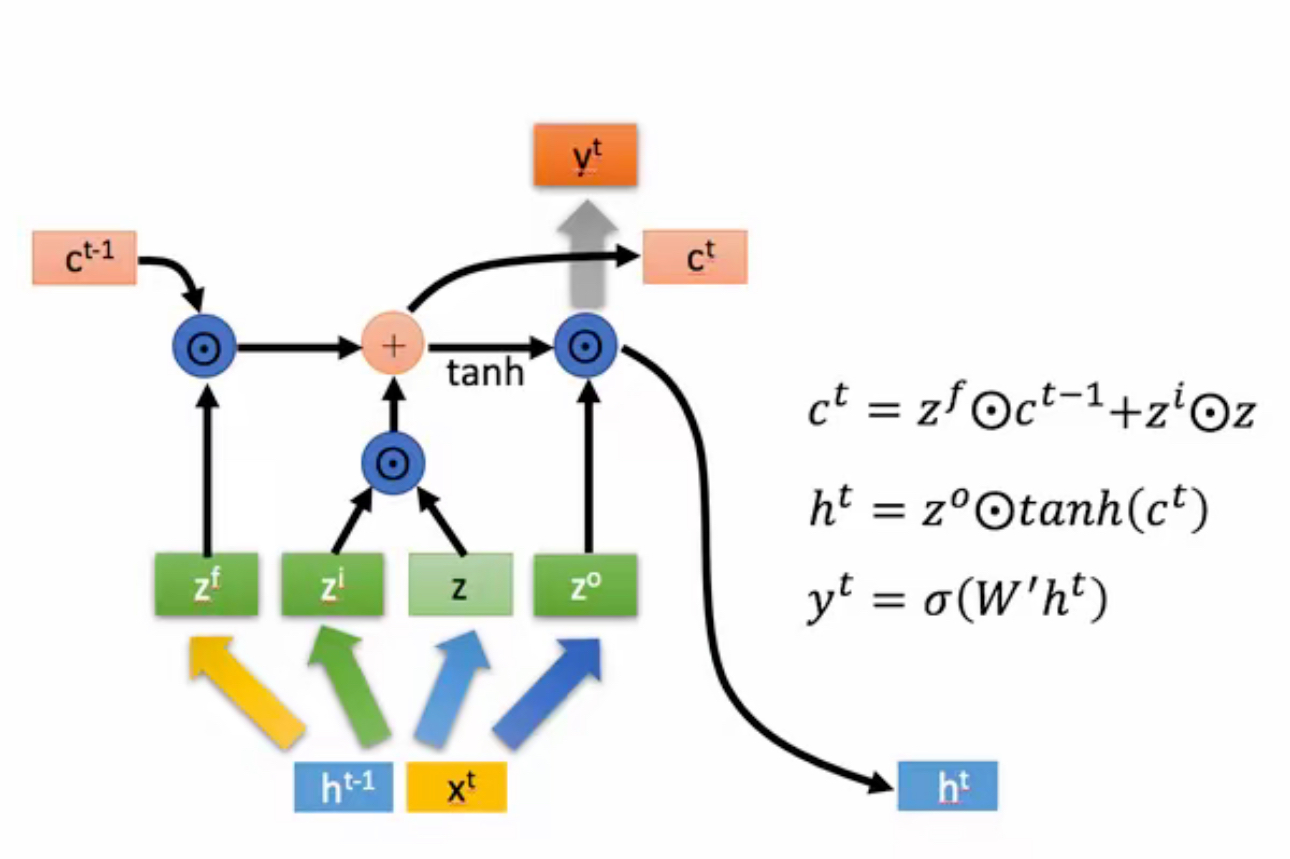
\includegraphics[width=\linewidth]{./img/lstm_structure.png} 
\caption{Structure of LSTM.}
\label{fig.1}
\end{center}
\end{figure}

The configuration of the LSTM model was optimized through hyperparameter tuning, including the number of LSTM layers, the number of units in each layer, the learning rate, and the batch size. The model was trained using the Adam optimizer and Mean Squared Error (MSE) as the loss function. The training process involved feeding the model with historical LOB data and iteratively updating the weights to minimize the loss.
The model was evaluated on a separate test set(the last 10\% of the whole data) to assess its predictive performance and generalization capabilities.
Below is the basic configuration of the LSTM model:
\begin{itemize}
    \item \textbf{Batch Size}: 256
    \item \textbf{Learning Rate}: 0.001
    \item \textbf{Epochs}: 50
    \item \textbf{Sequence Length}: 20
    \item \textbf{LSTM Layers}: 2
    \item \textbf{Hidden Size}: 256 units
    \item \textbf{Dropout Rate}: 0.2
\end{itemize}




\subsection{Trading Simulator Development}
Using the forecasts generated from the LSTM model, a trading simulator was constructed to simulate real-world trading. This simulator utilized the predictions to make trading decisions, attempting to maximize profits through strategic buy and sell orders. The trading strategy was based on a set of predetermined rules derived from the historical data patterns and predictive signals obtained from the model.

\subsubsection{Volatility}
The number of trades is adjusted based on current market volatility and risk tolerance to ensure trades are in line with the investor's risk tolerance.
Volatility is calculated from the rolling standard deviation of log returns.

\subsubsection{RSI}
The RSI (Relative Strength Index) is a momentum oscillator used to measure the speed and magnitude of changes in asset prices. It was developed by J. Welles Wilder Jr. in 1978 and is widely used in technical analysis. The RSI is designed to determine whether market conditions are overbought or oversold, providing traders with potential buy or sell signals.

First calculate the volume of price change:\[\Delta P = P_t - P_{t-1}\]

Then calculate the Average Gain and Average Loss:\[\text{Gain}_{\text{avg}} = \frac{\sum_{i=1}^{n} \max(\Delta P_i, 0)}{n}\]

\[\text{Loss}_{\text{avg}} = \frac{\sum_{i=1}^{n} \max(-\Delta P_i, 0)}{n}\]

Here \(n\) is the size of the rolling window and \(\Delta P_i\) is the price change at the \(i\) point in time.
Calculate Relative Strength:\[RS = \frac{\text{Gain}_{\text{avg}}}{\text{Loss}_{\text{avg}}}\]

Final calculation of RSI:\[RSI = 100 - \left(\frac{100}{1 + RS}\right)\\\]


\subsubsection{OFI}
OFI provides a measure of how the buying and selling power in a market changes over time, which can be used as a predictor of price movement. When OFI is positive, buyer power prevails; when OFI is negative, seller power prevails.


\Delta W^m\left(\tau_n\right)= \begin{cases}r^m\left(\tau_n\right), & \text { if } b^m\left(\tau_n\right)>b^m\left(\tau_{n-1}\right), \\ r^m\left(\tau_n\right)-r^m\left(\tau_{n-1}\right), & \text { if } b^m\left(\tau_n\right)=b^m\left(\tau_{n-1}\right), \\ -r^m\left(\tau_{n-1}\right), & \text { if } b^m\left(\tau_n\right)<b^m\left(\tau_{n-1}\right) ;
\end{cases}

\Delta V^m\left(\tau_n\right)= \begin{cases}-q^m\left(\tau_{n-1}\right), & \text { if } a^m\left(\tau_n\right)>a^m\left(\tau_{n-1}\right), \\ q^m\left(\tau_n\right)-q^m\left(\tau_{n-1}\right), & \text { if } a^m\left(\tau_n\right)=a^m\left(\tau_{n-1}\right), \\ q^m\left(\tau_n\right), & \text { if } a^m\left(\tau_n\right)<a^m\left(\tau_{n-1}\right);
\end{cases}

Where OFI is: e^m(\tau_n) = \Delta W^m(\tau_n) - \Delta V^m(\tau_n)



\subsection{Evaluation Metrics}
Model performance was assessed using several metrics:
\begin{itemize}
    \item \textbf{Mean Absolute Error (MAE)} for accuracy of predictions generated from regression model.
    \item \textbf{F1 Score} for performance of classification model.
    \item \textbf{Profitability}: The effectiveness of the trading simulator was measured by the profit generated during the simulation period.
\end{itemize}

\section{DATA DESCRIPTION/ PREPARATION}
\subsection{Data Description}
The data contains information on trading tapes (\emph{Tapes}) and limit order books (\emph{LOBs}) for a number of consecutive days. This data is used to analyse and model the behaviour of financial markets and to build trading simulators.

\textbf{Tapes:} Contains detailed information about each trade, such as the time of the trade, the number of trades, and the price at which they were executed. It is often used to refer to trading activity and data flow in the marketplace, especially the real-time quotes and transaction details of stock trades.

\textbf{LOB (Limit Order Book):} Records all open buy and sell orders in the market at a given moment. Each record contains the price, quantity, direction (buy or sell) of the order, the time the order was submitted and the exchange identification. In the financial markets, a limit order book is a mechanism for recording and ordering buy and sell orders on an exchange or trading platform. Each order specifies a price and quantity. Buy orders (the price at which to buy) will be listed in descending order, while sell orders (the price at which to sell) will be listed in descending order. This helps the trader to understand the supply and demand situation in the market, as well as the possible direction of price movements.

\subsection{Data Preparation}
Tape data is stored in csv format and LOB data is stored in txt format. Our first job is to parse the data and clean and merge it.

For Tape data, the date information contained in the file name is extracted directly and inserted as a new column in each file, and then all Tape data is merged in time order.

For LOB data, we wrote a Python script to parse the txt file, extract the date of the file name, and keep only Max Bid Price and Min Ask Price for each time point, which we think are the most important in LOB data, and also the most intuitive reflection of the market price trend. Accordingly, we keep the corresponding Max Bid Quantity and Min Ask Quantity, as well as the Total Bid/Ask Quantity for each time point, which can reflect the market depth information. Finally, all LOB files are merged to facilitate subsequent modelling.

We performed a simple data cleaning including removal of missing values, extraction of sliding window features as well as some features in the financial domain such as RSI, OFI (Order Flow Imbalance), etc., which were used as trading signals when we built the trading simulator later.



\subsection{References}

Please number citations consecutively within brackets \cite{b1}. The
sentence punctuation follows the bracket \cite{b2}. Refer simply to the reference
number, as in \cite{b3}---do not use ``Ref. \cite{b3}'' or ``reference \cite{b3}'' except at
the beginning of a sentence: ``Reference \cite{b3} was the first $\ldots$''

Capitalize only the first word in a paper title, except for proper nouns and
element symbols.

\section{Data Description / Preparation}
{\color{blue}Includes description of data sources, samples and steps for pre-processing if any.}

\section{Results and Discussion}
{\color{blue}Reporting on the experiments with discussion on insights. Technical challenges are to be discussed here too.}

\section{Further Work and Improvement}
{\color{blue}Explore what can be done further based on the discussed insights and ways to improve.}


\section{Conclusion}
{\color{blue}A brief summary of the key insights in your report.}

\begin{thebibliography}{00}
\bibitem{b1} G. Eason, B. Noble, and I. N. Sneddon, ``On certain integrals of Lipschitz-Hankel type involving products of Bessel functions,'' Phil. Trans. Roy. Soc. London, vol. A247, pp. 529--551, April 1955.
\bibitem{b2} J. Clerk Maxwell, A Treatise on Electricity and Magnetism, 3rd ed., vol. 2. Oxford: Clarendon, 1892, pp.68--73.
\bibitem{b3} I. S. Jacobs and C. P. Bean, ``Fine particles, thin films and exchange anisotropy,'' in Magnetism, vol. III, G. T. Rado and H. Suhl, Eds. New York: Academic, 1963, pp. 271--350.
\bibitem{b4} K. Elissa, ``Title of paper if known,'' unpublished.
\bibitem{b5} R. Nicole, ``Title of paper with only first word capitalized,'' J. Name Stand. Abbrev., in press.
\bibitem{b6} Y. Yorozu, M. Hirano, K. Oka, and Y. Tagawa, ``Electron spectroscopy studies on magneto-optical media and plastic substrate interface,'' IEEE Transl. J. Magn. Japan, vol. 2, pp. 740--741, August 1987 [Digests 9th Annual Conf. Magnetics Japan, p. 301, 1982].
\bibitem{b7} M. Young, The Technical Writer's Handbook. Mill Valley, CA: University Science, 1989.
\end{thebibliography}

\appendix
{\color{blue}The document up to this section should be no more than 8 pages. The appendix section is optional. You can include additional material here, but it will not be marked.}

\end{document}
